\chapter{Testy}
\label{chapter-5}

\vspace{0.5cm}

W rozdziale opisano kolejne etapy testowania urządzenia.

\FloatBarrier
\section{Testy}

Po złożeniu urządzenia przeprowadzono testy podstawowych funkcjonalności. Wyniki najważniejszych pomiarów przedstawiono 
w następnych podrozdziałach. Pomiary wartości prądu oraz napięcia dokonywane były multimetrami Uni-T UT60EU oraz UT107+.

\FloatBarrier
\subsection{Testy zasilacza regulowanego}

Przy pomocy zewnętrznego obciążenia aktywnego zweryfikowano działanie przetwornicy w module zasilacza regulowanego.
Zmierzono napięcie na wyjściu modułu dla trzech wybranych napięć (5 V, 9 V, 12 V, 15 V) oraz zakresu prądów od 0.1 A do 2 A. 
Zebrane dane przedstawiono w tabeli \ref{tab:pomiaryZasilacza}. Błąd względny obliczany jest ze wzoru: 
$\frac{V_{ustawione} - V_{zmierzone}}{V_{ustawione}} \cdot 100 \%$

\begin{table}[]
\centering
\begin{tabular}{|l|l|l|l|}
\hline
Napięcie ustawione {[}V{]} & Prąd wyjściowy {[}A{]} & Napięcie zmierzone {[}V{]} & Błąd względny {[}\%{]} \\ \hline
5                          & 0.1                    & 4.972                      & 0.56                   \\ \hline
5                          & 0.5                    & 4.94                       & 1.2                    \\ \hline
5                          & 1                      & 4.888                      & 2.24                   \\ \hline
5                          & 1.5                    & 4.832                      & 3.36                   \\ \hline
5                          & 2                      & 4.784                      & 4.32                   \\ \hline
9                          & 0.1                    & 8.992                      & 0.0889                 \\ \hline
9                          & 0.5                    & 8.956                      & 0.4889                 \\ \hline
9                          & 1                      & 8.904                      & 1.0667                 \\ \hline
9                          & 1.5                    & 8.848                      & 1.6889                 \\ \hline
9                          & 2                      & 8.802                      & 2.2                    \\ \hline
12                         & 0.1                    & 12.004                     & -0.0333                \\ \hline
12                         & 0.5                    & 11.965                     & 0.2917                 \\ \hline
12                         & 1                      & 11.916                     & 0.7                    \\ \hline
12                         & 1.5                    & 11.864                     & 1.1333                 \\ \hline
12                         & 2                      & 11.812                     & 1.5667                 \\ \hline
15                         & 0.1                    & 15.028                     & -0.1867                \\ \hline
15                         & 0.5                    & 14.998                     & 0.0133                 \\ \hline
15                         & 1                      & 14.936                     & 0.4267                 \\ \hline
15                         & 1.5                    & 14.888                     & 0.7467                 \\ \hline
15                         & 2                      & 14.852                     & 0.9867                 \\ \hline
\end{tabular}
\caption{Wyniki pomiarów modułu zasilacza regulowanego.}
\label{tab:pomiaryZasilacza}
\end{table}


\subsection{Testy obciążenia aktywnego}

Pomiary działania modułu obciążenia aktywnego wykonywano korzystając z zewnętrznego zasilacza laboratoryjnego PS-305D YIHUA.
Napięcie na zasilaczu ustawiono na 6 V oraz 12 V. Zmierzono pobierany przez moduł prąd dla kilku ustalonych wartości.
Zmierzone wartości przedstawia tabela \ref{tab:pomiaryObciazenia}. Błąd względny obliczany jest ze wzoru: 
$\frac{I_{ustawione} - I_{zmierzone}}{I_{ustawione}} \cdot 100 \%$
\begin{table}[]
\centering
\begin{tabular}{|l|l|l|l|}
\hline
Napięcie zasilacza {[}V{]} & Prąd ustawiony {[}A{]} & Prąd zmierzony {[}A{]} & Błąd względny {[}\%{]} \\ \hline
12                         & 0.1                    & 0.0994                 & 0.6                    \\ \hline
12                         & 0.5                    & 0.4945                 & 1.1                    \\ \hline
12                         & 1                      & 1.022                  & -2.2                   \\ \hline
12                         & 1.5                    & 1.514                  & -0.93333               \\ \hline
12                         & 2                      & 1.981                  & 0.95                   \\ \hline
6                          & 0.1                    & 0.0987                 & 1.3                    \\ \hline
6                          & 0.5                    & 0.4889                 & 2.22                   \\ \hline
6                          & 1                      & 1.001                  & -0.1                   \\ \hline
6                          & 1.5                    & 1.503                  & -0.2                   \\ \hline
6                          & 2                      & 1.992                  & 0.4                    \\ \hline
\end{tabular}
\caption{Wyniki pomiarów modułu obciążenia aktywnego.}
\label{tab:pomiaryObciazenia}
\end{table}



\subsection{Pomiar prądu i napięcia}

Sprawdzono również dokładność pomiaru prądu oraz napięcia, które dokonywane są w obu modułach poprzez układ INA219.
Wykorzystano w tym celu moduł zasilacza regulowanego do ustalania napięcia wyjściowego do pomiaru napięcia oraz 
moduł obciążenia aktywnego, w celu sprawdzenia dokładności pomiaru prądu. Tabele \ref{tab:pomiaryINA219} oraz 
\ref{tab:pomiaryINA2192} zawierają wyniki wykonanych pomiarów. Błąd względny liczony był analogicznie 
do pomiarów przedstawionych wcześniej.


\begin{table}[]
\centering
\begin{tabular}{|l|l|l|}
\hline
Napięcie zmierzone {[}V{]} & Napięcie rzeczywiste {[}V{]} & Błąd względny   {[}\%{]} \\ \hline
2.968                      & 2.978                        & -0.336             \\ \hline
4.988                      & 4.986                        & 0.040              \\ \hline
7.992                      & 8.001                        & -0.112             \\ \hline
11.004                     & 11.01                        & -0.054             \\ \hline
15.028                     & 15.05                        & -0.146             \\ \hline
19.04                      & 19.06                        & -0.105             \\ \hline
\end{tabular}
\caption{Pomiar napięcia przy pomocy układu INA219 oraz multimetru.}
\label{tab:pomiaryINA219}
\end{table}

\begin{table}[]
\centering
\begin{tabular}{|l|l|l|}
\hline
Prąd   zmierzony {[}A{]} & Prąd rzeczywisty   {[}A{]} & Błąd względny   {[}\%{]} \\ \hline
0.124                    & 0.121                      & 2.419              \\ \hline
0.241                    & 0.238                      & 1.244              \\ \hline
0.4                      & 0.399                      & 0.250                     \\ \hline
0.544                    & 0.541                      & 0.551              \\ \hline
0.841                    & 0.836                      & 0.594              \\ \hline
1.048                    & 1.042                      & 0.572              \\ \hline
1.267                    & 1.259                      & 0.631              \\ \hline
1.58                     & 1.567                      & 0.822               \\ \hline
1.812                    & 1.781                      & 1.710              \\ \hline
2.052                    & 2.01                       & 2.046             \\ \hline
\end{tabular}
\caption{Pomiar prądu przy pomocy układu INA219 oraz multimetru.}
\label{tab:pomiaryINA2192}
\end{table}




\subsection{Automatyczny pomiar sprawności przetwornicy}

Jednym z głównych celów projektu, jakie przedstawione zostały na początku tej pracy, była automatyzacja pomiaru sprawności 
przetwornic napięciowych. W tym celu, wytworzone oprogramowanie pozwala na wybór napięcia wejściowego oraz zakresu prądów obciążenia
przetwornicy. Następnie, po podłączeniu badanego układu (DUT), załączany jest moduł zasilacza regulowanego i ustalane napięcie wejściowe.
Obciążenie aktywne ustala następnie prąd wyjściowy DUT i oba moduły mierzą moc na swoich wejściach, tj. napięcie oraz prąd.
Po wykonaniu pomiaru, liczona jest sprawność, czyli stosunek mocy wejściowej i wyjściowej. Proces ten wykonywany jest dla
całego zakresu prądu obciążenia z wybranym krokiem. Po zakończeniu pomiarów, na wyświetlaczu urządzenia widoczny jest wykres
sprawności w podanym zakresie prądu obciążenia. Przykładowy wykonywany pomiar przedstawia zdjęcie \ref{fig:pomiarsprawnosci}.

\begin{figure}[h!]
    \begin{center}
        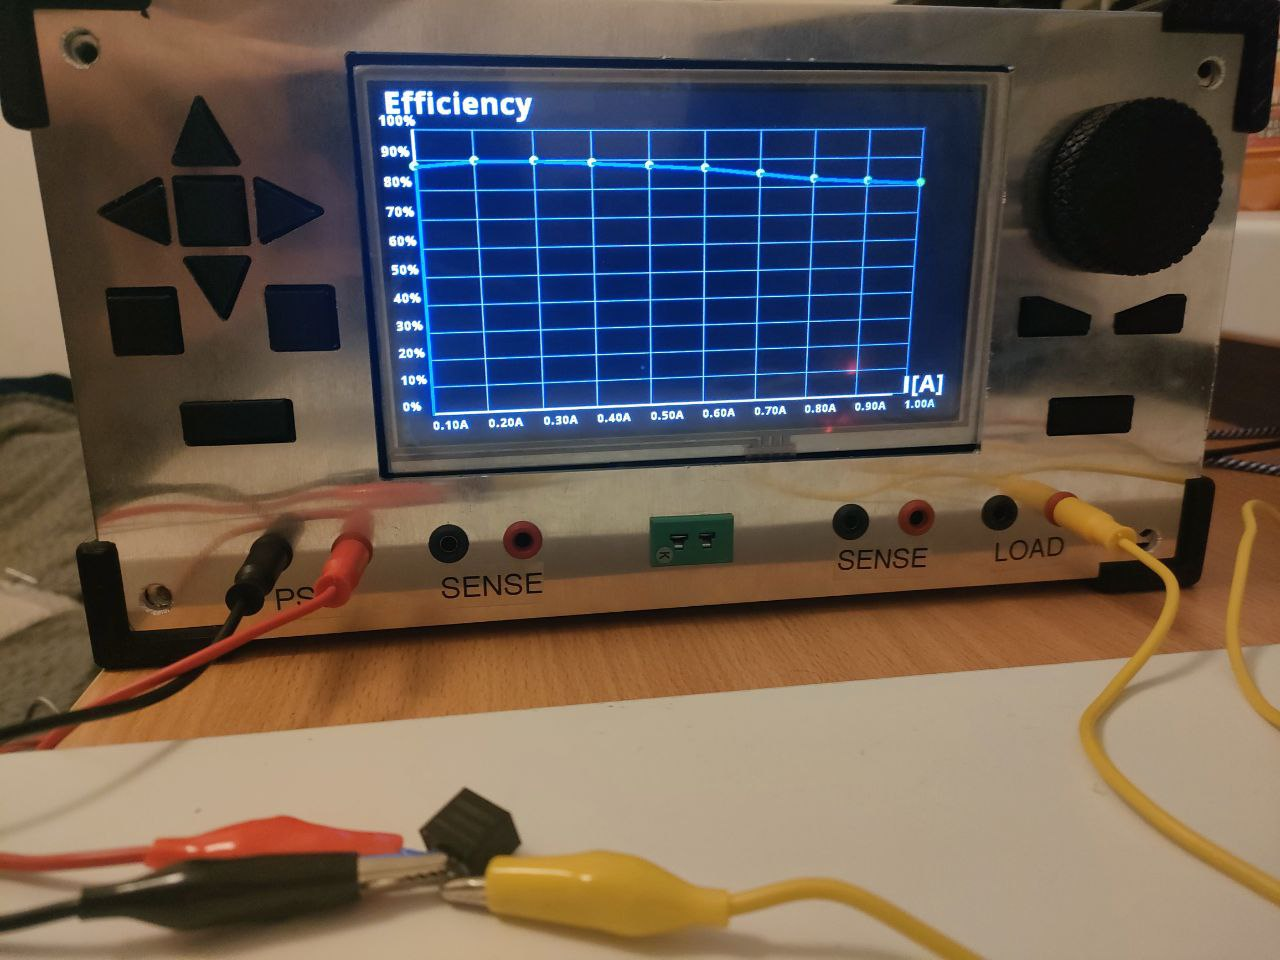
\includegraphics[width = 15cm]{images/pomiarSprawnosci.jpg}
        \caption{Automatyczny pomiar sprawności podłączonej przetwornicy.}
        \label{fig:pomiarsprawnosci}
    \end{center}
\end{figure}

Na zdjęciu widoczna jest przetwornica MORNSUN K7805-500R3 \cite{MORNSUN}. Jej napięcie wyjściowe to 5 V, natomiast maksymalny 
prąd to 500 mA. Pomiar wykonany został dla zakresu 0.1 A do 1 A, z krokiem 100 mA. Wartość 1 A przekracza oczywiście 
maksimum podane przez producenta, lecz testy wykazały stabilną pracę w temperaturze pokojowej do ponad 1 A, przy spadku 
napięcia wyjściowego do 4.4 V. Gwarantowany zakres 500 mA zakłada, że napięcie wyjściowe mieści się w zakresie 4\% od 
ustalonej wartości. 

Wykres \ref{fig:sprawnoscZmierzona} wygenerowany został z pomiarów w zakresie 0.05 A do 0.5 A prądu obciążenia, przy zasilaniu 
z napięcia 9 V.
Jest on analogiczny do wykresy przedstawionego na rysunku \ref{fig:sprawnoscOdProducenta}.

\begin{figure}[h!]
    \begin{center}
        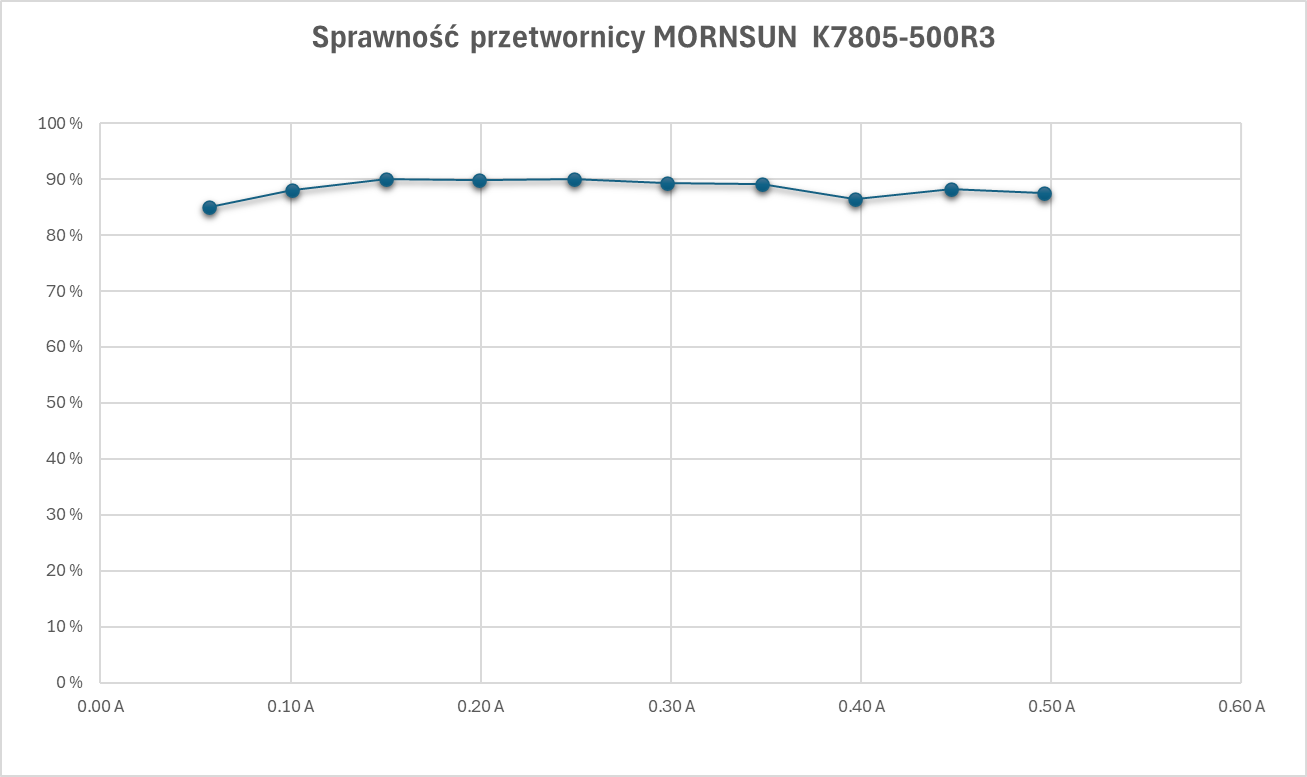
\includegraphics[width = 15cm]{images/sprawnoscZmierzonaMORNSUN.png}
        \caption{Wykres powstały ze zmierzonych wartości mocy przetwornicy MORNSUN.}
        \label{fig:sprawnoscZmierzona}
    \end{center}
\end{figure}

\begin{figure}[h!]
    \begin{center}
        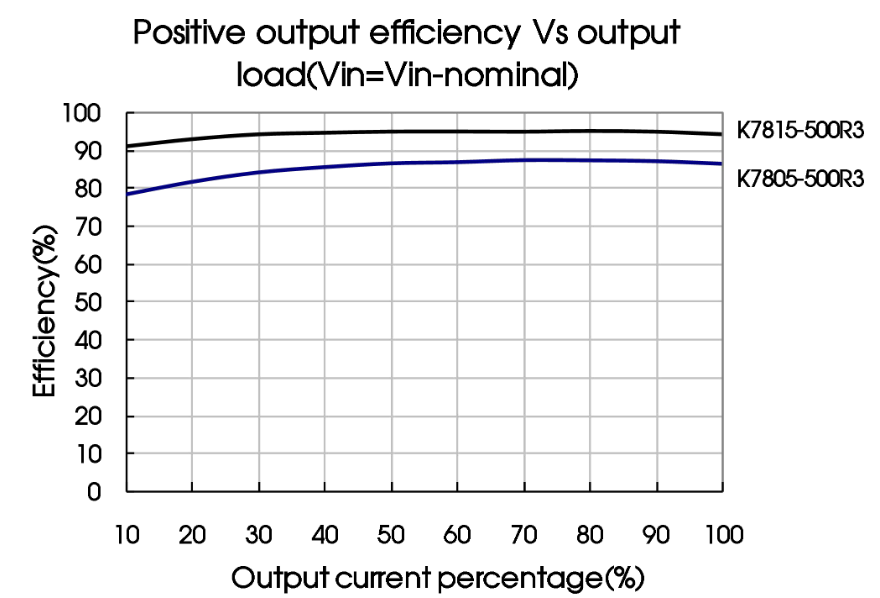
\includegraphics[width = 15cm]{images/sprawnoscProducentMORNSUN.png}
        \caption{Wykres sprawności przetwornicy MORNSUN z dokumentacji producenta.}
        \label{fig:sprawnoscOdProducenta}
    \end{center}
\end{figure}

Zarówno wykres z dokumentacji producenta, jak i wygenerowany z pomiarów, przedstawiają podobną krzywą sprawności.
Dla niewielkiego prądu wyjściowego sprawność wynosi około 85\% i wzrasta do prawie 90\% w połowie zakresu, po czym utrzymuje
ten poziom, aż do pełnego zakresu 500 mA.

